\documentclass[a4paper,12pt,italian]{article}
\usepackage{babel}
\usepackage[T1]{fontenc}
\usepackage[utf8]{inputenc}
\usepackage{amsmath}
\usepackage[margin=1.5cm]{geometry}
\usepackage{graphicx}

\title{
    Controlli Automatici T \\
    \large Progetto gruppo AO --- Traccia 3A\\
}
\author{
    Giacomo Romanini\\
    \and
    Guglielmo Palaferri\\
    \and
    Luca Tacinelli\\
    \and
    Pietro Girotti\\
}

\begin{document}
\maketitle

\begin{figure}[h]
    \begin{center}
        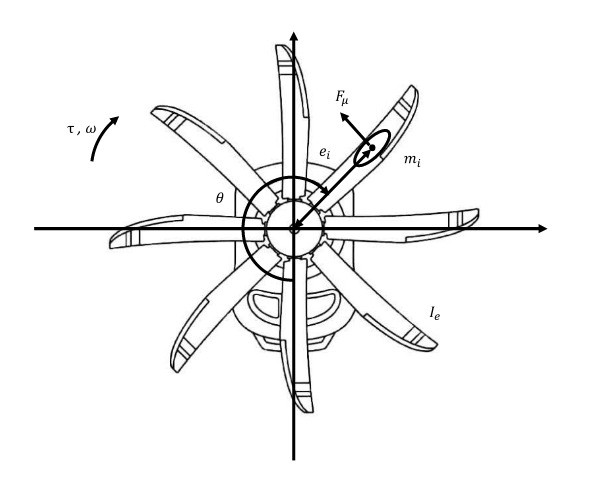
\includegraphics[scale=0.5]{img/elica.png}
        %\caption{Rappresentazione grafica del sistema (elica)}
    \end{center}    
\end{figure}

%\newpage

\section{Linearizzazione nell'intorno di $(x_e, u_e)$}
Il sistema del motore ad elica assegnato è descritto dalle seguenti equazioni: 

\begin{align*}
        \dot{\theta} &= \omega\\
        (m_i e_i^2 + I_e)\dot{\omega} &= -\beta \omega - \mu_d m_i \omega^2 e_i^2 + \tau
\end{align*}
Si considerano
\begin{align*}
    &x(t) =
    \begin{bmatrix}
        x_1(t)\\
        x_2(t)
    \end{bmatrix} =
    \begin{bmatrix}
        \theta(t)\\
        \omega(t)
    \end{bmatrix}\\
    &u(t) = \tau(t)\\
    &y(t) = \omega(t)
\end{align*}
Sostituendo i parametri è possibile ottenere le equazioni di stato:
\begin{equation*}
    \begin{aligned}
        \dot{x_1}(t) &= x_2(t)\\
        \dot{x_2}(t) &= -\frac{\beta}{(m_i e_i^2 + I_e)} x_2(t) - \frac{\mu_d m_i e_i^2}{(m_i e_i^2 + I_e)} x_2^2(t) + \frac{1}{(m_i e_i^2 + I_e)}u(t)
    \end{aligned}
\end{equation*} \\
Inoltre, poiché la dinamica di $\theta$ è ininfluente per l'evoluzione del sistema, si conosce $x_e = 
\begin{pmatrix}
    0\\
    10000/2\pi
\end{pmatrix}$
e $y_e = \omega_e = 10000/2\pi$.
$u_e$ può essere calcolato ponendo $f_2(x_e, u_e) = 0$:
\begin{equation*}
    -\beta x_{2e} - \mu_d m_i e_i^2 x_{2e}^2 + u_e = 0 \hspace{1em} \Longrightarrow \hspace{1em} u_e \approx 1110.7222
\end{equation*}
Si procede a questo punto calcolando le matrici del sistema linearizzato:
\begin{equation*}
    \delta \dot{x}(t) = A\delta x(t) + B\delta u(t)
\end{equation*}
\begin{equation*}
    \begin{array}{ll}
    A = \frac{\partial f(x,u)}{\partial x} \bigg|_{\substack{x=x_e\\u=u_e}} =
    \begin{bmatrix} 
        0 & 1 \\ 
        0 & - \frac{\beta}{m_ie_i^2 + I_e} - \frac{\mu_dm_ie_i^2}{m_ie_i^2 + I_e} 2\omega_e 
    \end{bmatrix}
    &B = \frac{\partial f(x,u)}{\partial u} \bigg|_{\substack{x=x_e\\u=u_e}} = 
    \begin{bmatrix} 
        0 \\ 
        \frac{1}{m_ie_i^2 + I_e}
    \end{bmatrix}\\ \\
    C = \frac{\partial h(x,u)}{\partial x} \bigg|_{\substack{x=x_e\\u=u_e}} =
    \begin{bmatrix} 
        0 & 1
    \end{bmatrix}
    &D = \frac{\partial h(x,u)}{\partial u} \bigg|_{\substack{x=x_e\\u=u_e}} =
    \begin{bmatrix} 
        0
    \end{bmatrix}
    \end{array}
\end{equation*}

%\newpage

\section{Funzione di trasferimento}

Per calcolare la funzione di trasferimento, si utilizza l'espressione
\begin{equation*}
    G(s) = C(sI - A)^{-1}B + D
\end{equation*}
dove
\begin{equation*}
    (sI - A)^{-1} = \frac{adj(sI - A)}{det(sI - A)} = 
    \begin{bmatrix}
        1/s & \frac{1}{s(s + 1.4139)} \\ 
        0   & \frac{1}{s + 1.4139}
    \end{bmatrix}
\end{equation*}
Ottenendo quindi la funzione di trasferimento:
\begin{equation*}
    G(s) =
    \begin{bmatrix}0 & 1 \end{bmatrix}
    \begin{bmatrix}
        1/s & \frac{1}{s(s+1.4139)} \\
        0 &\frac{1}{s+1.4139} \end{bmatrix}
    \begin{bmatrix}0 \\ 1.2903 \end{bmatrix}
    + 0 =
    \frac{1.2903}{s + 1.4139}
\end{equation*}
Avendo un polo in $s = -1.4139$, è possibile constatare con certezza che il sistema sia BIBO stabile.\\ \\
Di seguito il diagramma di Bode della funzione di trasferimento, ricavato tramite MATLAB.

\begin{figure}[h!]
    \begin{center}
        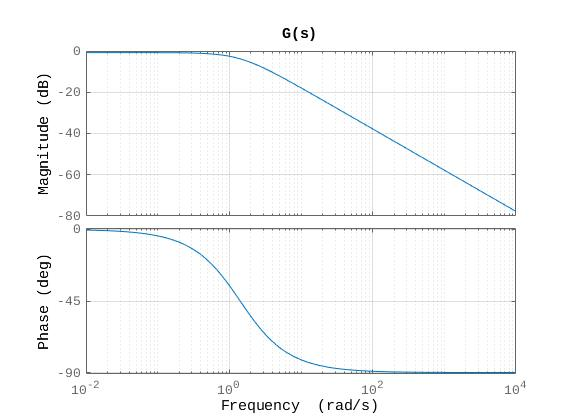
\includegraphics[scale=0.55]{img/bode_GG.jpg}
        %\caption{Rappresentazione grafica del sistema (elica)}
    \end{center}    
\end{figure}

\newpage

\section{Specifiche del regolatore}

\textbf{(3.1)} Per ottenere un errore a regime nullo con riferimento a gradino $w(t) = W1(t)$, $L(s)$ deve presentare un polo nell'origine.
Avendo un unico polo reale negativo, possiamo introdurre a questo scopo un regolatore statico con un polo nell'origine: $ R_s(s) = \frac{1}{s} $ ricavandone quindi $ G_e(s) $:

\begin{equation*}
    G_e(s) = R_s(s)G(s) = \frac{1}{s}\Big(\frac{1.2903}{s + 1.4139}\Big)
\end{equation*}

\textbf{(3.2)} Come si può notare, il sistema esteso rispetta le specifiche iniziali sul margine di fase ($ M_f \geq 45^\circ$)\\

\textbf{(3.3)} La sovraelongazione percentuale massima accettabile è pari all'1\%. 
Da questo ricaviamo un nuovo vincolo sul margine di fase, sapendo che $M_f = \xi \cdot 100 $

\begin{equation*}
    \begin{array}{c}
        \xi^* = \sqrt{\frac{(ln(0.01))^2}{\pi^2+(ln(0.01))^2}} = 0.8261\\ \\
        M_f=\xi * 100 \Longrightarrow M^*_{f,min}=0.8261 \cdot 100 = 82.61
        \Longrightarrow arg(L(j\omega_c)) \geq -97.39^\circ
    \end{array}
\end{equation*}\\
Il nuovo vincolo sul margine di fase introduce quindi un minimo non rispettato dal sistema esteso.\\

\textbf{(3.4)} Il tempo di assestamento all'1\% deve essere mantenuto al di sotto dei 6 secondi.
Posso quindi ottenere $ \omega_{c,min} $

\begin{equation*}
    T_{a,1} = 6 
    \Longrightarrow 
    \omega_c \ge \frac{460}{6 \cdot 82.61}
    \Longrightarrow
    \omega_c \ge 0.9281
\end{equation*}

%\newpage

\textbf{(3.5)} Considerando variazioni del parametro $e_i$ di $\pm 0.1$, si ottiene il seguente diagramma:

\begin{figure}[h!]
    \begin{center}
        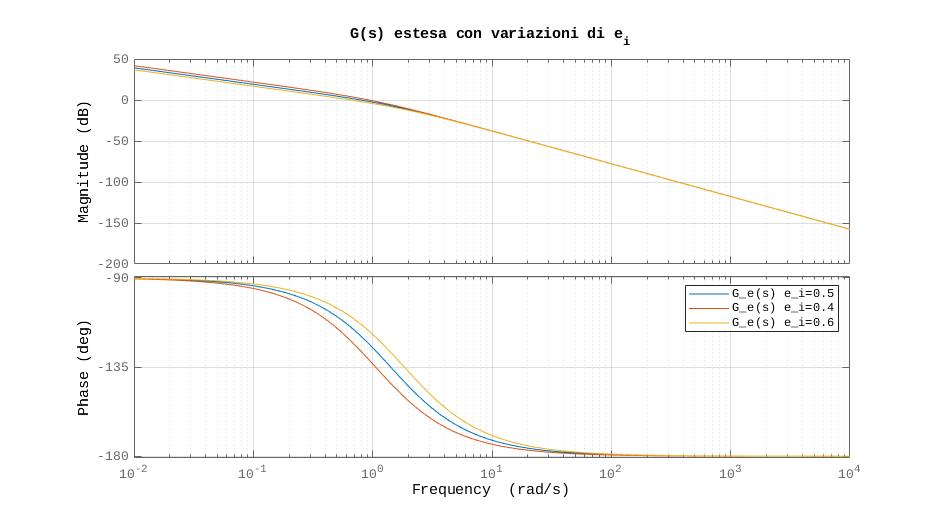
\includegraphics[scale=0.5]{img/bode_GG_estesa_ei.jpg}
    \end{center}    
\end{figure}

\newpage

\section{Disturbo di misura}

Il disturbo di misura presenta componenti frequenziali maggiori di 100 rad/s e deve essere abbattuto di almeno 30 volte.
Di conseguenza a frequenze $\omega \geq 100~rad/s$, il grafico di $L(j\omega)$ non potrà avere ampiezze maggiori di $-30dB$.\\ \\
Di seguito il diagramma di Bode del sistema esteso con i vincoli ottenuti dalle specifiche.

\begin{figure}[h!]
    \begin{center}
        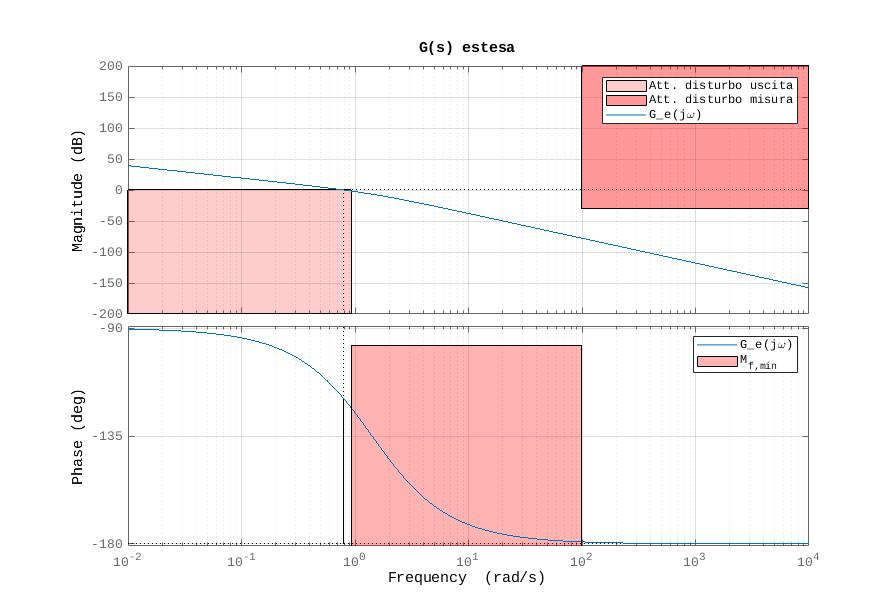
\includegraphics[scale=0.5]{img/bode_GG_estesa.jpg}
    \end{center}    
\end{figure}
Come si può notare, sia le specifiche sull'ampiezza che quelle sul margine di fase non vengono rispettate.
In particolare notiamo che, se anche $\omega_c$ si trovasse nel range $[\omega_{c,min}, \omega_{c,max}]$,
le specifiche sul margine di fase non sarebbero rispettate.
Possiamo ricondurci dunque ad uno scenario di tipo B.


\section*{Sintesi del regolatore dinamico}

Poiché ci interessa un anticipo di fase minore di $90^\circ$, 
per soddisfare le specifiche è sufficiente introdurre una rete anticipatrice con uno zero:

\begin{equation*}
    R_d(s)= \mu_d \frac{1+\tau s} { 1 + \alpha \tau s} 
\end{equation*}\\
Procedendo in maniera empirica abbiamo scelto $\omega_c^* = 1.2281~rad/s$, 
valutando poi argomento ed ampiezza di $G_e$ in $\omega_c^*$:

\begin{equation*}
        arg(G_e(J w^*_c))= -130.9762^\circ
        \hspace{2em}|G_e(J w^*_c)|dB = -5.0201 dB
\end{equation*}\\
A questo punto possiamo calcolare $\phi^*$ ed $M^*$:
\begin{equation*}
    \varphi^*_c=(M^*_fmin +5)-180-(\space-arg(G_e(J w^*_c))\space)=38.5862
    \hspace{2em}
    M^*=10^\frac{-|Ge(Jw_c^*)|dB}{20}=1.7824
\end{equation*}

Ottenendo infine i valori di $\tau$ ed $\alpha \tau$ per determinare l'espressione di $R_d(s)$

\begin{equation*}
    \tau = \frac{M^*-cos(\varphi^*)}{\omega^*_c\cdot sin(\varphi^*)}
         = 1.2087
    \hspace{2em}
    \alpha \tau = \frac{cos(\varphi^*)-\frac{1}{M^*}}{\omega_c^*sin(\varphi^*)}
                = 0.1064
\end{equation*}\\
\begin{equation*}
    R_d(s) = 1.95\frac{1+1.2087s}{1+0.1064s}
\end{equation*}

L'espressione finale di L(s) sarà quindi:

\begin{equation*}
    L(s) = R_d(s) G_e(s) = 
    1.95
    \frac{1+1.2087s}{1+0.1064s}~
    \frac {1} {s}
    \bigg(\frac { 1.2903 }{s+1.4139}\bigg)
    = \frac{28.58(s+0.8273)}{s(s+9.4)(s+1.4139)}
\end{equation*}

\begin{figure}[h!]
    \begin{center}
        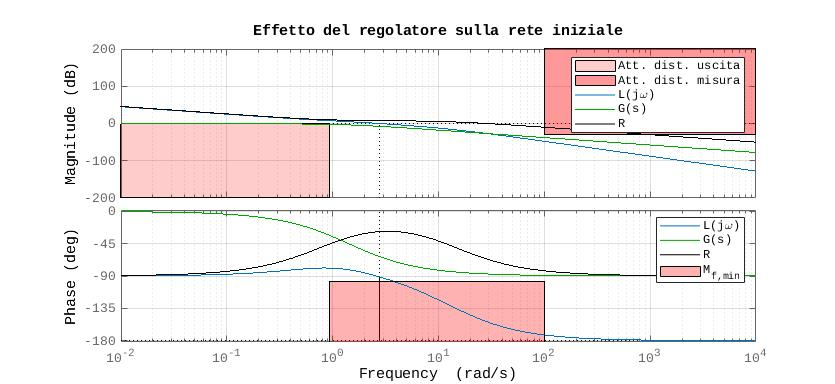
\includegraphics[scale=0.6]{img/bode_GG_RR_LL.jpg}
    \end{center}
\end{figure}

\begin{figure}[h!]
    \begin{center}
        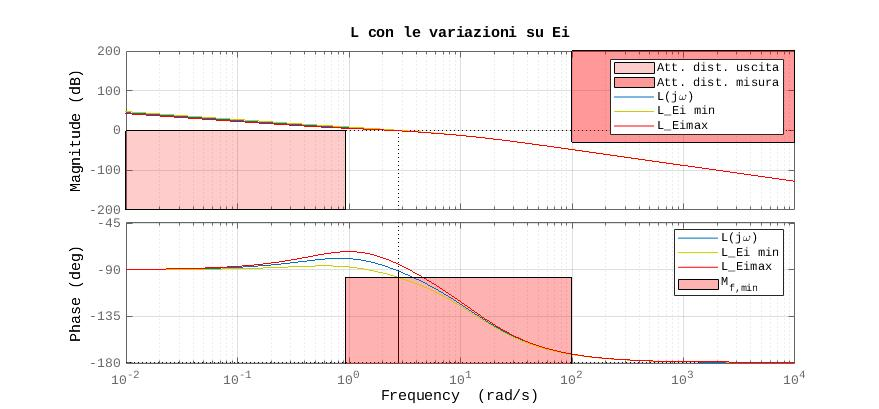
\includegraphics[scale=0.58]{img/bode_LL_ei.jpg}
    \end{center}
\end{figure}

\newpage

\begin{figure}[h!]
    \begin{center}
        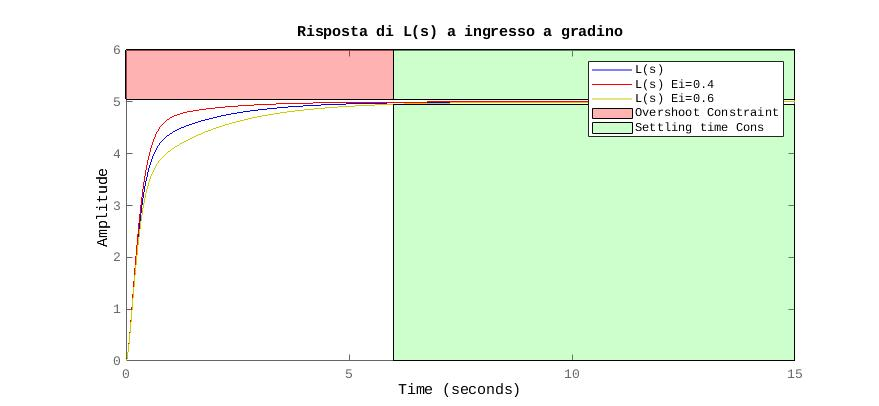
\includegraphics[scale=0.58]{img/step_LL_ei.jpg}
    \end{center}
\end{figure}

\section{Test del regolatore}

Mediante Simulink è possibile testare il regolatore sul modello non lineare (in allegato il file simulink).
Il modello è stato testato fornendo un ingresso a gradino di ampiezza $W=5$ al tempo $t=1$

\begin{figure}[h!]
    \centering
    \begin{minipage}{0.45\textwidth}
        \centering
        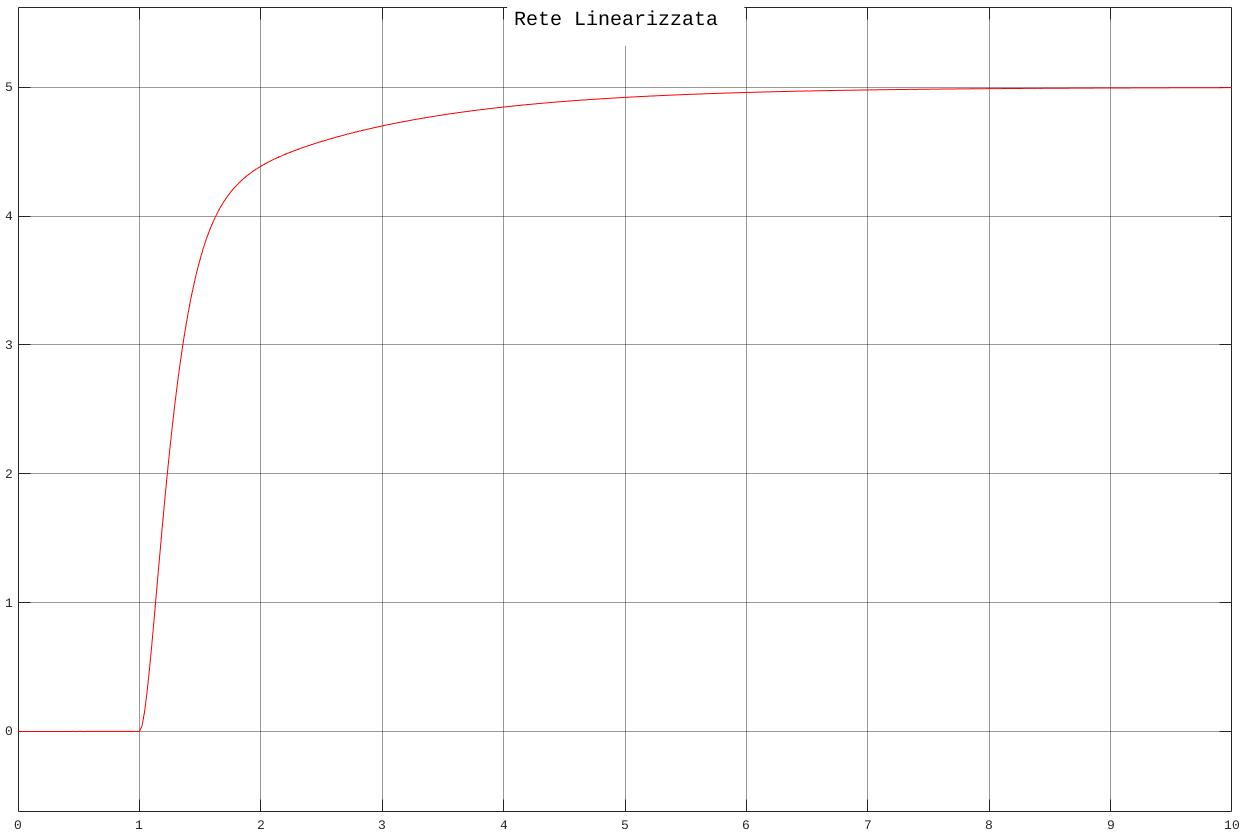
\includegraphics[scale=0.2]{img/modello_lineare.jpg}
        \caption{Rete linearizzata}
    \end{minipage}\hspace{2em}
    \begin{minipage}{0.45\textwidth}
        \centering
        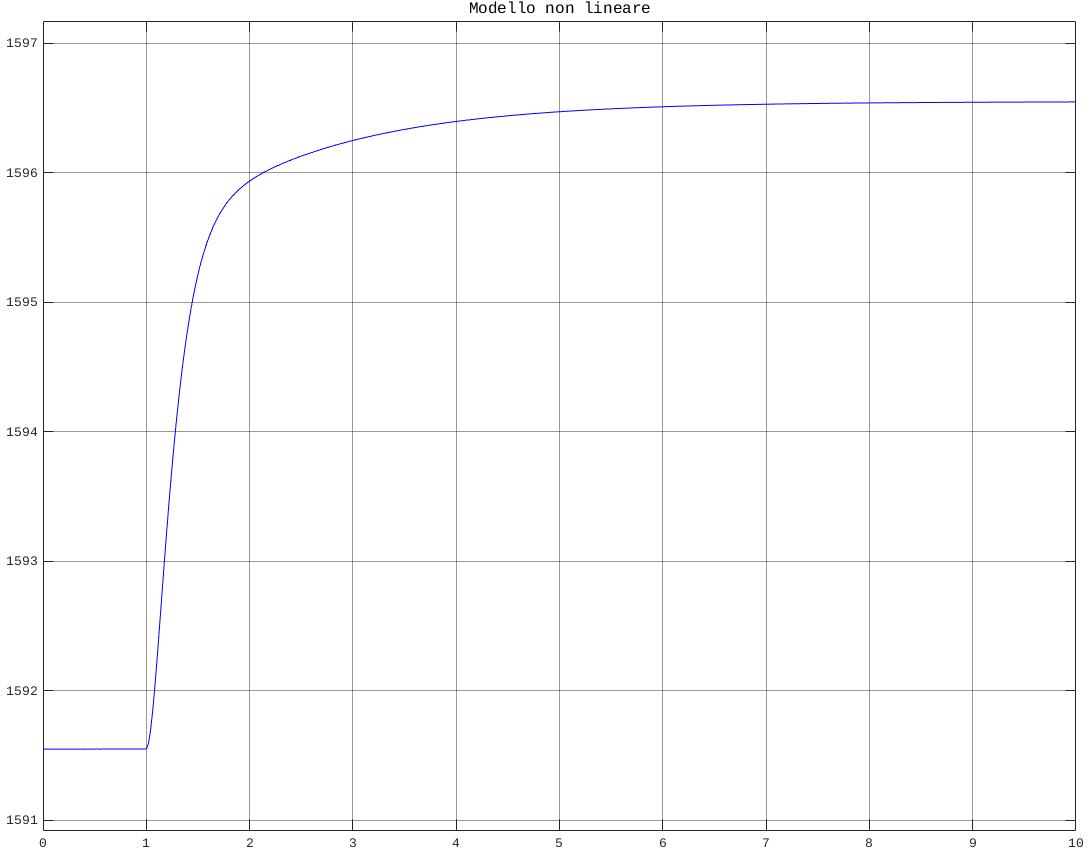
\includegraphics[scale=0.23]{img/modello_non_lineare.jpg}
        \caption{Modello non lineare}
    \end{minipage}
\end{figure}

Come si può osservare, la rete non lineare risponde ai test riproducendo quasi perfettamente il comportamento della rete lineare.

\newpage

\section{Punti opzionali}

\textbf{(6.2)} Testando il modello non lineare con condizioni iniziali nell'intorno del punto di equilibrio, il sistema risponde nel modo atteso.
Impostando invece velocità iniziali molto elevate (in particolare con ${\omega_0 >7\cdot10^5~rad/s}$), il sistema inizia a rispondere in modo anomalo,
producendo un'uscita di questo tipo:

\begin{figure}[h!]
    \begin{center}
        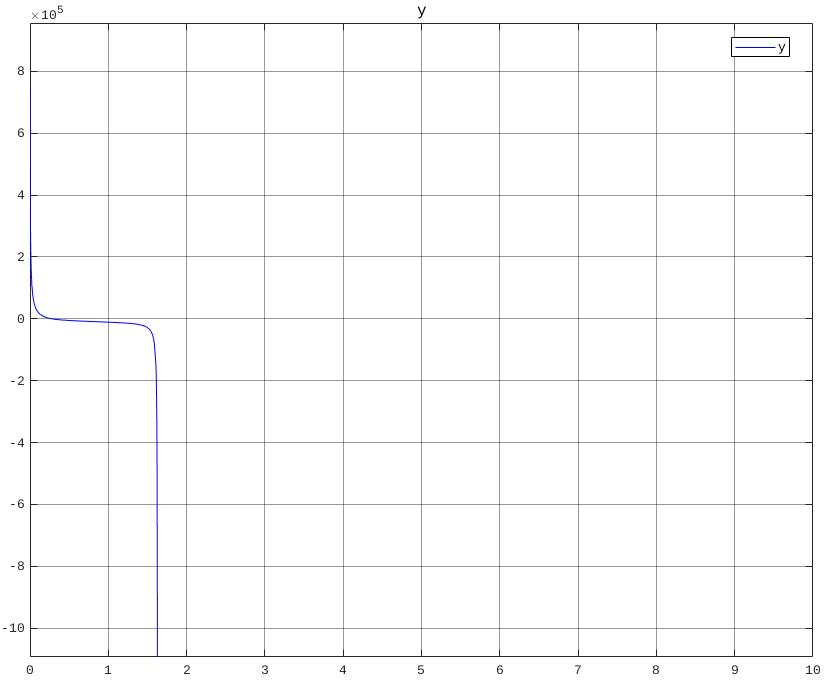
\includegraphics[scale=0.35]{img/risposta_omega_iniz_elevato.jpg}
    \end{center}
\end{figure}
In questo caso una risposta anomala era in parte prevedibile per via della velocità iniziale estremamente elevata.\\ \\
\textbf{(6.3)}
Nel testare il sistema con variazioni del valore di riferimento W, abbiamo riscontrato una situazione simile a quella del punto precedente.
Nonostante il sistema non presenti anomalie particolari anche per riferimenti W molto alti, il vincolo sul tempo di assestamento all'1\% (6 secondi) cessa di essere soddisfatto per riferimenti $W > 2150$

\begin{figure}[h!]
    \begin{center}
        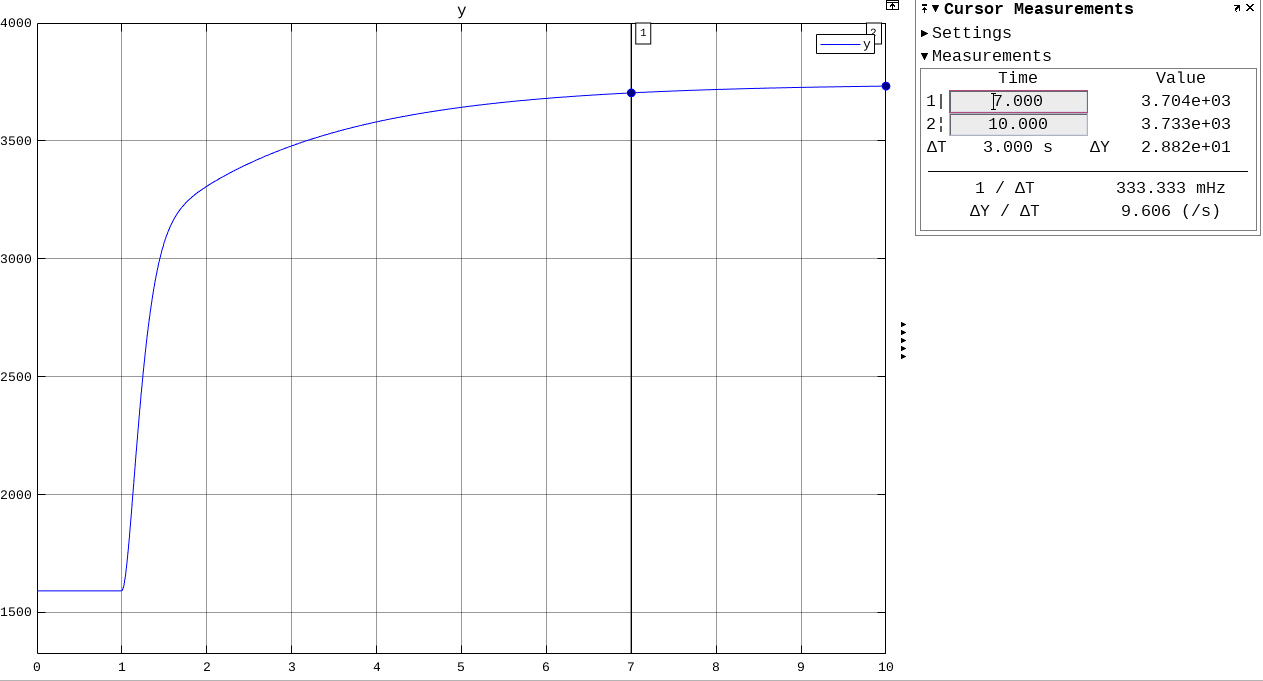
\includegraphics[scale=0.35]{img/variazioni_W.png}
        \caption{Risposta del sistema ad un riferimento $W = 2150$}
    \end{center}
\end{figure}

\end{document}